\documentclass[12pt,a4paper,fleqn]{article}
\usepackage{rmpackages}																% usual packages
\usepackage{rmtemplate}																% graphic charter
\usepackage{rmexocptce}																% for DS with cptce eval

%\cfoot{} 													% if no page number is needed
%\renewcommand\arraystretch{1.5}		% stretch table line height

\begin{document}

\begin{header}
Chapitre 6 -- Exercices
\end{header}

\section*{Corrections}

\subsection*{Exercice 4 page 160}

\begin{center}
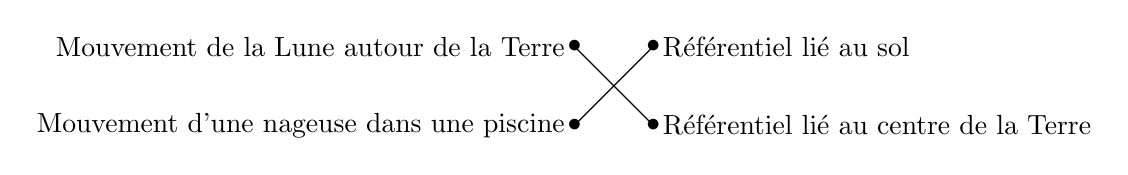
\begin{tikzpicture}
\draw (0,0) node {$\bullet$};
\draw (0,1) node {$\bullet$};
\draw (1,0) node {$\bullet$};
\draw (1,1) node {$\bullet$};
\draw (0,1) node [left] {Mouvement de la Lune autour de la Terre} -- (1,0) node [right] {Référentiel lié au centre de la Terre};
\draw (0,0) node [left] {Mouvement d'une nageuse dans une piscine} -- (1,1) node [right] {Référentiel lié au sol};
\end{tikzpicture}
\end{center}

\subsection*{Exercice 7 page 160}

La modélisation du skieur par un point entraine une perte d'information.
Le point C passe à côté de la porte donc, avec ce modèle, il n'y a aucun problème car on ne prend pas en compte les bras du skieur.

\subsection*{Exercice 9 page 161}

\begin{enumerate}
\item La personne sur le tapis roulant est immobile dans le \textbf{référentiel lié au tapis roulant}.
\item La personne sur le tapis roulant est en mouvement dans le référentiel :
\begin{itemize}
\item[•] lié au sol ;
\item[•] lié au banc ;
\item[•] lié à la personne qui marche.
\end{itemize}
\item \textbf{Le mouvement d'un système dépend du référentiel choisi !}
\end{enumerate}

\subsection*{Exercice 12 page 161}

Cf. correction page 312.

\subsection*{Exercice 13 page 161}

Caractéristique du vecteur vitesse représenté sur le schéma :
\begin{itemize}
\item[•] direction : horizontale ;
\item[•] sens : vers la droite ;
\item[•] norme : $v = \unit{40}{km\per h}$.
\item[•] (point d'origine : le centre du bus.)
\end{itemize}

\subsection*{Exercice 14 page 161}

\begin{itemize}
\item[(a)] Mouvement rectiligne et uniforme.
\item[(b)] Mouvement curviligne accéléré (première moitié du mouvement) puis décéléré (deuxième moitié du mouvement).
\item[(c)] Mouvement rectiligne et accéléré.
\end{itemize}

\subsection*{Exercice 19 page 162}

\begin{enumerate}
\item Il faut déterminer la longueur des vecteur à tracer compte tenu de la norme de $\vec{v_1}$ et $\vec{v_2}$ et de l'échelle indiquée dans l'énoncé. Pour $\vec{v_1}$ par exemple :
\begin{center}
\begin{tabular}{c|c}
\unit{1}{cm} & \unit{2}{m/s} \\
\hline
? & \unit{3{,}0}{m/s}
\end{tabular}
\end{center}
La longueur $l_1$ du vecteur à tracer sera pour $\vec{v_1}$ :
\[
l_1 = \frac{1\times 3{,}0}{2} = \unit{1{,}5}{cm}.
\]
De même pour $\vec{v_2}$, on trouve $l_2 = \unit{2{,}5}{cm}$.

\begin{center}
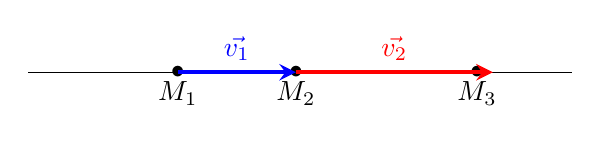
\begin{tikzpicture}
\coordinate (O) at (0,0);
\coordinate (Z) at (6.9,0);
\coordinate (A) at (1.9,0);
\coordinate (B) at (3.4,0);
\coordinate (C) at (5.7,0);
\draw (O) -- (Z);
\draw (A) node [below] {$M_1$};
\draw (A) node {$\bullet$};
\draw (B) node [below] {$M_2$};
\draw (B) node {$\bullet$};
\draw (C) node [below] {$M_3$};
\draw (C) node {$\bullet$};
\draw [->, >= stealth, color=blue, ultra thick] (A) --++ (1.5, 0) node [midway, above] {$\vec{v_1}$};
\draw [->, >= stealth, color=red, ultra thick] (B) --++ (2.5, 0) node [midway, above] {$\vec{v_2}$};
\end{tikzpicture}
\end{center}

\item Le mouvement est rectiligne et accéléré.
\end{enumerate}

\subsection*{Exercice 21 page 162}

\begin{enumerate}
\item Le système étudié est le passager du manège.

Le référentiel d'étude est le référentiel lié au sol.

\item Le mouvement est circulaire et uniforme.

\item La vitesse du passager est \unit{60}{km/h}.
Compte tenu de l'échelle utilisée pour représenter les vecteurs vitesse, il faudra tracer des vecteur de \unit{3}{cm} de long.

\begin{center}
\begin{tikzpicture}
\newcommand{\radius}{3}

\coordinate (O) at (0,0);
\coordinate (A) at (90:\radius);
\coordinate (B) at (210:\radius);
\coordinate (C) at (330:\radius);

\draw (O) node {$\bullet$};
\draw (O) node [below left] {$O$};
\draw [dashed] (O) circle (\radius);

\draw [->, >= stealth, color=blue, ultra thick] (A) node {$\times$} --++ (180:3) node [midway, above] {$\vec{v_1}$};
\draw [->, >= stealth, color=red, ultra thick] (B) node {$\times$} --++ (300:3) node [midway, left] {$\vec{v_2}$};
\draw [->, >= stealth, color=green, ultra thick] (C) node {$\times$} --++ (60:3) node [midway, right] {$\vec{v_3}$};
\end{tikzpicture}
\end{center}

\item La direction et le sens du vecteur vitesse changent au cours du temps (ainsi que son point de départ) mais la norme reste constante.
\end{enumerate}

\subsection*{Exercice 22 page 163}

\begin{enumerate}
\item
\begin{enumerate}
\item Les radars tronçon permettent de mesurer la vitesse moyenne d'un véhicule.

Les autres radars permettent de mesurer la vitesse instantanée.

\item Ces vitesses sont mesurées dans le référentiel lié au sol.
\end{enumerate}

\item Dans le document 2, on lit :
\begin{itemize}
\item[•] $d=\unit{6}{km} = \unit{6000}{m} = \unit{6\times10^3}{m}$ ;
\item[•] 14h 28min 50s - 14h 25min 50s = 3 min : $\Delta t = \unit{3}{min} = \unit{180}{s}$.
\end{itemize}
\[
v = \frac{d}{\Delta t} = \frac{6000}{180} \approx \unit{33{,}3}{m/s}.
\]
La vitesse moyenne de l'automobiliste sur le tronçon concerné est $v = \unit{33{,}3}{m/s}$.

\item Pour répondre à cette question, il faut exprimer la vitesse de l'automobiliste en km/h :
\begin{itemize}
\item[•] \textbf{Méthode 1 :} en calculant directement la vitesse en km/h.
\[
\Delta t = \unit{3}{min} = \unit{\frac{3}{60}}{h} = \unit{0{,}05}{h} \text{ car il y a 60 minnutes dans une heure}
\]
donc
\[
v = \frac{d}{\Delta t} = \frac{6 \text{\,\color{gray_f}km}}{0{,}05 \text{\,\color{gray_f}h}} = \unit{120}{km/h}.
\]

\item[•] \textbf{Méthode 2 :} en convertissant la vitesse trouvée précédemment en km/h.
\[
v = \unit{33{,}3}{m/s} \xrightarrow{\times 3600} \unit{120\,000}{m/h} \xrightarrow{\div 1000} \unit{120}{km/h}
\]
\end{itemize}
La vitesse de l'automobiliste est donc \unit{120}{km/h} ce qui est en dessous de la limitation de vitesse sur autoroute par temps sec (\unit{130}{km/h}).
L'automobiliste n'est pas verbalisable par ce radar tronçon.
\end{enumerate}

\subsection*{Exercice 31 page 165}

\begin{enumerate}
\item La direction et le sens du vecteur vitesse ne changent pas mais sa norme augmente (et le point de départ se déplace avec le système).

\item C'est un mouvement rectiligne accéléré.

\item On veut déterminer la valeur de la vitesse en $M_5$, c'est-à-dire la norme du vecteur $\vec{v_5}$.

Sur le schéma on mesure la longueur du vecteur $\vec{v_5}$ et on trouve \unit{6}{mm}.
L'échelle des vecteurs vitesse nous indique que \unit{4}{mm} correspondent à \unit{20}{m/s}.
\begin{multicols}{2}
\begin{center}
\begin{tabular}{c|c}
\unit{4}{mm} & \unit{20}{m/s} \\
\hline
\unit{6}{mm} & $v_5$
\end{tabular}
\end{center}
\[
v_5 = \frac{6 \times 20}{4} = \unit{30}{m/s}
\]
\end{multicols}
On convertit cette valeur en km/h :
\[
v = \unit{30}{m/s} \xrightarrow{\times 3600} \unit{108\,000}{m/h} \xrightarrow{\div 1000} \unit{108}{km/h}.
\]

La vitesse en $M_5$ est plus petite que \unit{122}{km/h} mais le plongeur a encore plus de \unit{20}{m} à parcourir avant de toucher l'eau, pendant lesquels il continue d'accélérer.
Il est donc normal de trouver en $M_5$ un valeur de vitesse plus faible que celle indiquée dans l'article.
\end{enumerate}

\end{document}